\documentclass[tikz,border=4pt]{standalone}
% Estilo común de los diagramas de bloques (se usa con \input en cada standalone)
\usepackage[defaultsans,scale=0.92]{lato}
\usepackage{libertinust1math}
\usepackage{xcolor,amsmath}
\usepackage{tikz}
\usetikzlibrary{positioning,arrows.meta,calc,shapes.geometric}
\usepackage{../../notacion}
\definecolor{ctrlazul}{HTML}{1E5AA8}\definecolor{ctrlnoche}{HTML}{14213D}
\definecolor{ctrlcoral}{HTML}{D1495B}\definecolor{ctrlverde}{HTML}{2A9D8F}
\definecolor{ctrlambar}{HTML}{E09F3E}\definecolor{ctrlgris}{HTML}{5C677D}
\definecolor{ctrlvioleta}{HTML}{6C4AB6}\definecolor{ctrlteal}{HTML}{0F7173}
\tikzset{
  >={Stealth[length=2.4mm]}, every node/.style={font=\small},
  bloque/.style={draw=ctrlnoche,fill=ctrlazul!7,thick,rounded corners=1.5pt,minimum height=9mm,minimum width=13mm,inner sep=4pt},
  suma/.style={draw=ctrlnoche,thick,circle,inner sep=0pt,minimum size=6mm},
  senal/.style={->,thick,draw=ctrlnoche},
  rot/.style={font=\footnotesize,text=ctrlgris},
}

\begin{document}
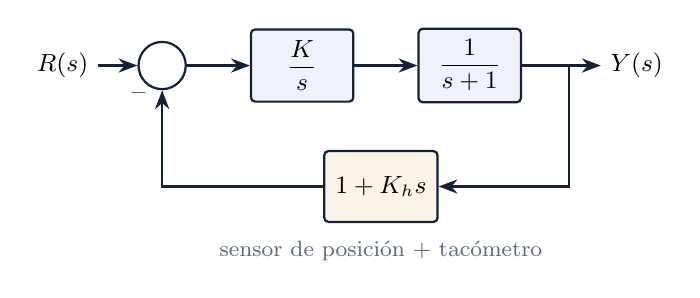
\begin{tikzpicture}[node distance=8mm]
  \node (r) {$R(s)$}; \node[suma,right=5mm of r] (S) {};
  \node[bloque,right=of S] (k) {$\dfrac{K}{s}$}; \node[bloque,right=of k] (p) {$\dfrac{1}{s+1}$};
  \coordinate[right=6mm of p] (o); \node[right=4mm of o] (y) {$Y(s)$};
  \node[bloque,below=6mm of k,xshift=10mm,fill=ctrlambar!12] (h) {$1+K_h s$};
  \draw[senal] (r)--(S); \draw[senal] (S)--(k); \draw[senal] (k)--(p); \draw[thick,draw=ctrlnoche] (p)--(o); \draw[senal] (o)--(y);
  \draw[senal] (o)|-(h); \draw[senal] (h)-|(S); \node[rot] at ($(S)+(-3mm,-3.5mm)$) {$-$};
  \node[rot,below=1mm of h] {sensor de posición + tacómetro};
\end{tikzpicture}
\end{document}
